\documentclass{article}
\usepackage{tikz}
\usepackage{amsmath,amssymb,bm}

\begin{document}

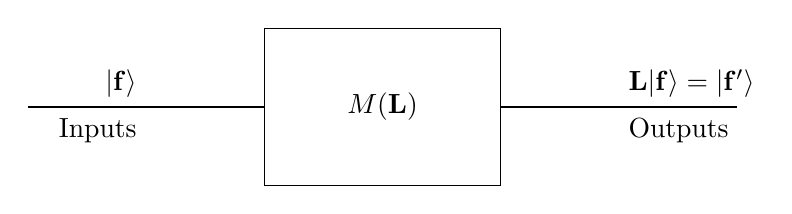
\begin{tikzpicture}
    % Define the box for the computing machine
    \draw (0,0) rectangle (3,2);
    
    % Add the label for the computing machine
    \node at (1.5,1) {$M(\mathbf{L})$};
    
    % Draw input line
    \draw (-3,1) -- (0,1);
    
    % Draw output line
    \draw (3,1) -- (6,1);
    
    % Add input label
    \node[left] at (-1.5,1.3) {$|{\bf f}\rangle$};
    \node[left] at (-1.5,0.7) {Inputs};
    
    % Add output label
    \node[right] at (4.5,1.3) {$\mathbf{L}|{\bf f}\rangle = |{\bf f}'\rangle$};
    \node[right] at (4.5,0.7) {Outputs};
    
\end{tikzpicture}

\end{document}